
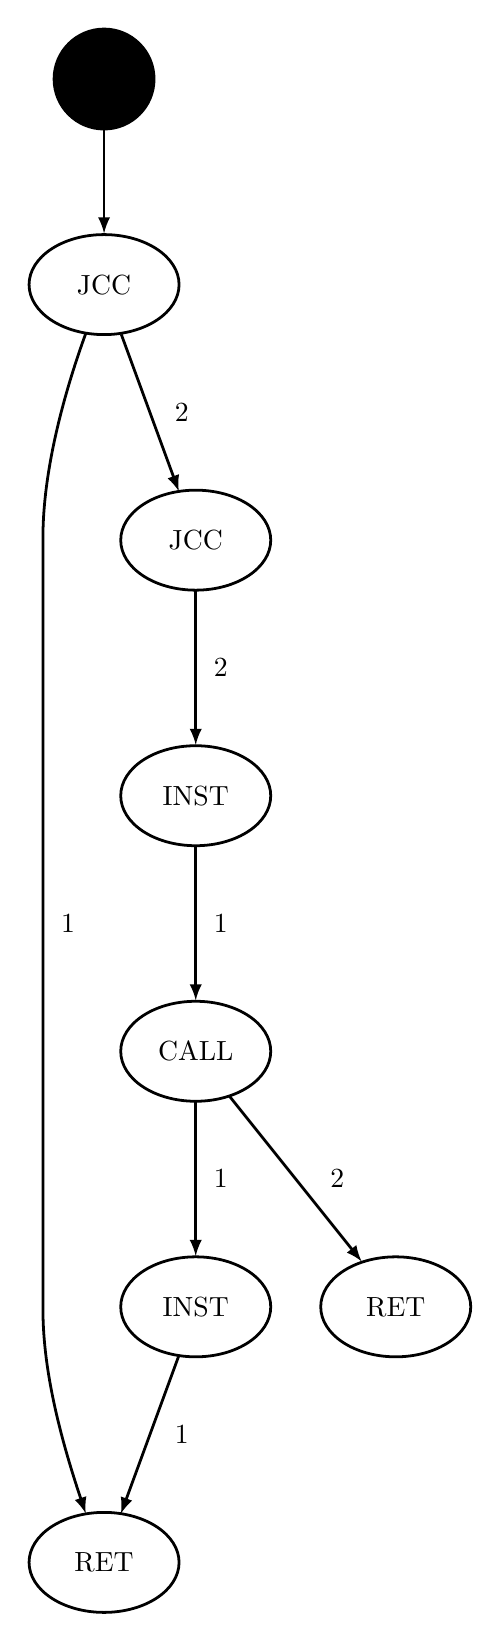
\begin{tikzpicture}[>=latex,line join=bevel,]
  \pgfsetlinewidth{1bp}
%%
\pgfsetcolor{black}
  % Edge: 2 -> 3
  \draw [->] (60.0bp,183.65bp) .. controls (60.0bp,170.82bp) and (60.0bp,153.11bp)  .. (60.0bp,128.3bp);
  \definecolor{strokecol}{rgb}{0.0,0.0,0.0};
  \pgfsetstrokecolor{strokecol}
  \draw (69.0bp,156.0bp) node {1};
  % Edge: 6 -> 7
  \draw [->] (60.0bp,367.65bp) .. controls (60.0bp,354.82bp) and (60.0bp,337.11bp)  .. (60.0bp,312.3bp);
  \draw (69.0bp,340.0bp) node {2};
  % Edge: 1 -> 6
  \draw [->] (33.207bp,460.07bp) .. controls (38.031bp,446.92bp) and (44.809bp,428.43bp)  .. (53.932bp,403.55bp);
  \draw (55.0bp,432.0bp) node {2};
  % Edge: 7 -> 2
  \draw [->] (60.0bp,275.65bp) .. controls (60.0bp,262.82bp) and (60.0bp,245.11bp)  .. (60.0bp,220.3bp);
  \draw (69.0bp,248.0bp) node {1};
  % Edge: 1 -> 4
  \draw [->] (20.399bp,460.38bp) .. controls (13.919bp,442.54bp) and (5.0bp,413.22bp)  .. (5.0bp,387.0bp) .. controls (5.0bp,387.0bp) and (5.0bp,387.0bp)  .. (5.0bp,109.0bp) .. controls (5.0bp,87.083bp) and (11.233bp,63.0bp)  .. (20.399bp,35.622bp);
  \draw (14.0bp,248.0bp) node {1};
  % Edge: 0 -> 1
  \draw [->] (27.0bp,533.94bp) .. controls (27.0bp,525.81bp) and (27.0bp,515.88bp)  .. (27.0bp,496.44bp);
  % Edge: 2 -> 5
  \draw [->] (72.214bp,185.73bp) .. controls (83.488bp,171.64bp) and (100.4bp,150.5bp)  .. (119.73bp,126.34bp);
  \draw (111.0bp,156.0bp) node {2};
  % Edge: 3 -> 4
  \draw [->] (53.793bp,92.072bp) .. controls (48.969bp,78.915bp) and (42.191bp,60.429bp)  .. (33.068bp,35.548bp);
  \draw (55.0bp,64.0bp) node {1};
  % Node: 1
\begin{scope}
  \definecolor{strokecol}{rgb}{0.0,0.0,0.0};
  \pgfsetstrokecolor{strokecol}
  \draw (27.0bp,478.0bp) ellipse (27.0bp and 18.0bp);
  \draw (27.0bp,478.0bp) node {JCC};
\end{scope}
  % Node: 0
\begin{scope}
  \definecolor{strokecol}{rgb}{0.0,0.0,0.0};
  \pgfsetstrokecolor{strokecol}
  \definecolor{fillcol}{rgb}{0.0,0.0,0.0};
  \pgfsetfillcolor{fillcol}
  \filldraw [opacity=1] (27.0bp,552.0bp) ellipse (18.0bp and 18.0bp);
\end{scope}
  % Node: 3
\begin{scope}
  \definecolor{strokecol}{rgb}{0.0,0.0,0.0};
  \pgfsetstrokecolor{strokecol}
  \draw (60.0bp,110.0bp) ellipse (27.0bp and 18.0bp);
  \draw (60.0bp,110.0bp) node {INST};
\end{scope}
  % Node: 2
\begin{scope}
  \definecolor{strokecol}{rgb}{0.0,0.0,0.0};
  \pgfsetstrokecolor{strokecol}
  \draw (60.0bp,202.0bp) ellipse (27.0bp and 18.0bp);
  \draw (60.0bp,202.0bp) node {CALL};
\end{scope}
  % Node: 5
\begin{scope}
  \definecolor{strokecol}{rgb}{0.0,0.0,0.0};
  \pgfsetstrokecolor{strokecol}
  \draw (132.0bp,110.0bp) ellipse (27.0bp and 18.0bp);
  \draw (132.0bp,110.0bp) node {RET};
\end{scope}
  % Node: 4
\begin{scope}
  \definecolor{strokecol}{rgb}{0.0,0.0,0.0};
  \pgfsetstrokecolor{strokecol}
  \draw (27.0bp,18.0bp) ellipse (27.0bp and 18.0bp);
  \draw (27.0bp,18.0bp) node {RET};
\end{scope}
  % Node: 7
\begin{scope}
  \definecolor{strokecol}{rgb}{0.0,0.0,0.0};
  \pgfsetstrokecolor{strokecol}
  \draw (60.0bp,294.0bp) ellipse (27.0bp and 18.0bp);
  \draw (60.0bp,294.0bp) node {INST};
\end{scope}
  % Node: 6
\begin{scope}
  \definecolor{strokecol}{rgb}{0.0,0.0,0.0};
  \pgfsetstrokecolor{strokecol}
  \draw (60.0bp,386.0bp) ellipse (27.0bp and 18.0bp);
  \draw (60.0bp,386.0bp) node {JCC};
\end{scope}
%
\end{tikzpicture}

